\documentclass{article}
\usepackage{amsmath}
\usepackage{tikz}
\title{Quantum Mechanics}
\author{Author}
\date{\today}
\begin{document}
\maketitle
\section{Equations}
The Schrödinger equation:
\begin{equation}
 i\hbar \frac{\partial}{\partial t} \Psi = \hat{H} \Psi
\end{equation}
This is missing a closing brace above.
\begin{figure}[h!]
    \centering
    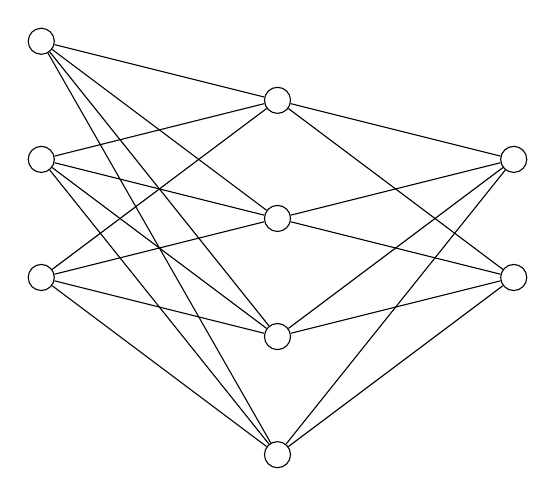
\begin{tikzpicture}[scale=1.5]
        % Input layer
        \foreach \i in {1,...,3} \node[circle, draw] (input\i) at (0, -\i) {};
        % Hidden layer
        \foreach \i in {1,...,4} \node[circle, draw] (hidden\i) at (2, -\i-0.5) {};
        % Output layer
        \foreach \i in {1,...,2} \node[circle, draw] (output\i) at (4, -\i-1) {};
        % Connections
        \foreach \i in {1,...,3} \foreach \j in {1,...,4} \draw (input\i) -- (hidden\j);
        \foreach \i in {1,...,4} \foreach \j in {1,...,2} \draw (hidden\i) -- (output\j);
    \end{tikzpicture}
    \caption{Simple Neural Network}
    \label{fig:neural_network}
\end{figure}
\section{Results}
The results are summarized below.
\end{document}